\documentclass[dvipdfmx]{jarticle}
\usepackage{graphicx}
\usepackage[top=30truemm,bottom=30truemm,left=25truemm,right=25truemm]{geometry}
\usepackage{listings,jvlisting}

\lstset{
  basicstyle={\ttfamily},
  identifierstyle={\small},
  commentstyle={\smallitshape},
  keywordstyle={\small\bfseries},
  ndkeywordstyle={\small},
  stringstyle={\small\ttfamily},
  frame={tb},
  breaklines=true,
  columns=[l]{fullflexible},
  numbers=left,
  xrightmargin=0zw,
  xleftmargin=3zw,
  numberstyle={\scriptsize},
  stepnumber=1,
  numbersep=1zw,
  lineskip=-0.5ex
}

\begin{document}
\begin{titlepage}
    \begin{center}
        {\huge 情報科学演習C 課題4レポ―ト}
        \vspace{180pt}\\
        \begin{tabular}{rl}
            氏名 & 山久保孝亮\\
            所属 & 大阪大学基礎工学部情報科学科ソフトウェア科学コース\\
            メールアドレス & u327468b@ecs.osaka-u.ac.jp\\
            学籍番号 & 09B22084\\
            提出日 & \today\\
            担当教員 & 平井健士,中島悠太
        \end{tabular}
    \end{center}
\end{titlepage}
\section{課題4-1}
\subsection{プログラムの仕様}
課題4-1で作成したクライアントプログラムchatclient.cの仕様は以下の通りである.
\begin{itemize}
    \item プログラム実行の書式は"./chatclient [サーバプログラムを実行中のホスト名] [使用したいユーザ名]"である.
    \item 接続できたかどうか,名前を登録できたかどうかが標準出力に表示される.接続できた場合はチャット機能が使用でき,接続できなかった場合はプログラムが終了する.
    \item チャット機能には以下の3つの機能がある.
    \begin{enumerate}
        \item 標準入力に文字列を書き込んで[Enter]キーを押すと,サーバにその文字列を送信する.
        \item サーバに接続されているほかのホストから送られてきた文字列を受信し,標準入力に表示させる.
        \item EOFを入力するとサーバとの接続が切れ,プログラムを終了する.
    \end{enumerate}
\end{itemize}
また,サーバプログラムchatserver.cの仕様は以下の通りである.
\begin{itemize}
    \item プログラム実行の書式は引数はなしである.即ち"./chatserver"である.
    \item 一度に接続できるユーザの数は5つである.
    \item 常に新たなユーザの接続を待っており,新たに接続しようとするユーザが現れた場合には正常に接続できたかどうかと,すでに同じユーザ名が登録されていないかを確認する.どちらも
    満たしていればその旨の文字列を送信して新たなユーザとして登録し,いずれかを満たさない場合はその旨の文字列を送信して再び待ち状態に入る.
    \item 登録されたユーザから文字列を受信した場合は,その文字列の先頭にユーザ名を追加して送信してきたユーザ以外に追加した後の文字列を送信する.
    \item EOFを受信するとそのユーザの接続を切り,ユーザの情報を削除する.
\end{itemize}
また,両社のプログラムに共通する仕様は以下のとおりである.
\begin{itemize}
    \item 使用するポート番号は10140である.
    \item ユーザ名は英数字,ハイフン,アンダースコアのみから成る.
\end{itemize}
\subsection{クライアントプログラムのアルゴリズム}
今回作成したプログラムは指導書の状態に則って作成しており,以下の図1のフローチャートはそれぞれの状態の遷移の様子を表す.
\begin{figure}[h]
    \centering
    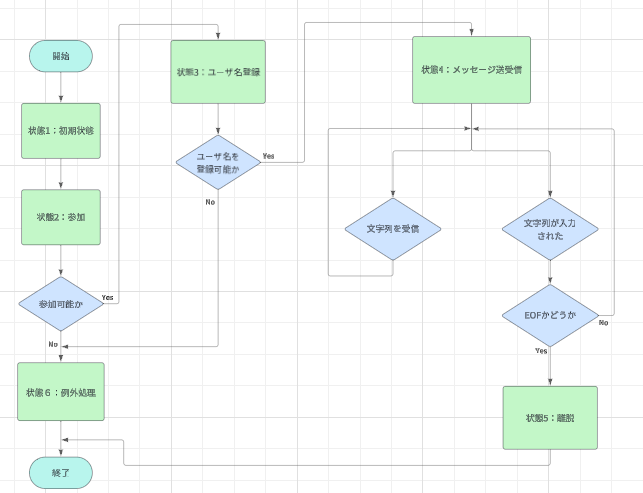
\includegraphics[width=8cm]{4-1clienthurotya.png}
    \caption{クライアントプログラムのフローチャート}
\end{figure}
\\それぞれの状態は指導書のとおりに実装した.また,図1には無いがそれぞれの状態の処理で異常が発生した場合は状態6として例外処理が存在する.それぞれの状態の概要は以下のとおりである.
\begin{description}
    \item[状態1:初期状態]  \\  ソケットを作成し,第一引数のホスト名に接続要求を出す.
    \item[状態2:参加] \\ サーバから接続できたかどうかの文字列を受け取る.
    \item[状態3:ユーザ名登録] \\ 第二引数のユーザ名を送信し,ユーザ名を登録できたかどうかの文字列を受け取る.
    \item[状態4:メッセージ送受信] \\ 標準入力から文字列が入力されればその文字列をサーバへ送信する.サーバから文字列を受信すればその文字列を標準入力へ出力する.
    \item[状態5:離脱] \\ 標準入力が"EOF"のとき,ソケットを閉じてプログラムを正常終了する.
    \item[状態6:例外処理] \\ サーバに接続拒否またはユーザ名の登録に失敗した際に,ソケットを閉じてプログラムを異常終了する.
\end{description}
\subsection{クライアントプログラムの実装方法}
ここではアルゴリズムで記述した各状態とその条件分岐の詳細な実装方法について記述する.
以下の表1はこのプログラムで使用した変数名とその表す内容である.
\begin{table}[h]
    \centering
    \begin{tabular}{|c|c|c|}
        \hline
        変数名 & 型 & 表す内容\\\hline\hline
        sock & int & ソケットディスクリプタ\\\hline
        n & int & 入出力操作の結果を格納\\\hline
        rbuf[1024] & char & 送受信する文字列を格納\\\hline
        rfds & fd\_set & ファイルディスクリプタのセット\\\hline
        tv & struct timeval & タイムアウト値を設定する構造体\\\hline
        *server & struct hostent & ホスト情報を格納するためのポインタ\\\hline
        svr & struct sockaddr\_in & サーバのアドレス情報を格納する構造体\\\hline
        current\_time & time\_t & 現在の時刻を格納\\\hline
        *local\_time & struct tm & ローカルタイムを表す構造体へのポインタ\\\hline
        argc & int & 引数の個数を格納\\\hline
        *argv[] & char & 引数の文字列を格納\\\hline
    \end{tabular}
    \caption{このプログラムで使用した変数}
\end{table}
\subsubsection{初期状態}
状態1のプログラムは大きく以下のように処理が分かれる.
\begin{enumerate}
    \item 書式の確認し,ソケットを作成
    \item ホスト名を取得し,接続する
\end{enumerate}
以下でその詳細について記述する.
\begin{enumerate}
    \item この処理のプログラムは以下のようになる.
\begin{lstlisting}
if(argc != 3){
    fprintf(stderr, "Usage: %s <hostname> <username>\n", argv[0]);
    exit(1);
}
if ((sock=socket(AF_INET,SOCK_STREAM,IPPROTO_TCP))<0) {
    perror("socket");
    exit(1);
}
\end{lstlisting}
コマンドライン引数が3であるかどうかを確認して書式が正しいかを確認する.ここでargcの値が3である理由は"./chatclient"も引数として数えられるためである.
そしてsock()を使ってソケットを作成する.
    \item この処理のプログラムは以下のようになる.
\begin{lstlisting}
server = gethostbyname(argv[1]);
if (server == NULL) {
    fprintf(stderr, "ERROR, no such host as %s\n", argv[1]);
    exit(0);
}
bzero((char *)&svr, sizeof(svr));
svr.sin_family = AF_INET;
bcopy((char *)server->h_addr, (char *)&svr.sin_addr.s_addr, server->h_length);
svr.sin_port = htons(10140);
if (connect(sock, (struct sockaddr *)&svr, sizeof(svr)) < 0) {
    perror("client: connect");
    close(sock);
    exit(1);
}
\end{lstlisting}
コマンドライン引数の1番目の引数をホスト名として変数に格納する.ここでインデックスが1である理由はargv[0]に"./chatclient"が格納されているからである.
そしてそのホスト名のサーバがあればconnect()を使って接続をサーバに要請する.
\end{enumerate}
\subsubsection{参加と参加できたかどうかの条件分岐}
状態2のプログラムは以下のようになる.
\begin{lstlisting}
bzero(rbuf, 1024);
n = read(sock, rbuf, 1024);
if(n <= 0){
    perror("Connection closed by client.\n");
    close(sock);
    return 0;
}else if(strcmp(rbuf,"REQUEST ACCEPTED\n") == 0) {
状態3の処理
}else{
状態6の処理}
\end{lstlisting}
1から2行目でサーバから文字列を受信する.正常に受信ができればその内容が"REQUEST ACCEPTED \textbackslash n"と一致しているかどうかを確認し一致していれば状態3へ,一致していなければ状態6へ遷移する.
文字列が一致しているかどうかの判定にはstrcmp()を使用した.
\subsubsection{ユーザ名登録}
状態3のプログラムは大きく以下のように処理が分かれる.
\begin{enumerate}
    \item 書式の確認し,ソケットを作成
    \item ホスト名を取得し,接続する
\end{enumerate}
\subsubsection{メッセージ送受信}
状態4のプログラムは大きく以下のように処理が分かれる.
\begin{enumerate}
    \item 書式の確認し,ソケットを作成
    \item ホスト名を取得し,接続する
\end{enumerate}
\subsubsection{離脱}
状態5のプログラムは以下のようになる.
\begin{lstlisting}
printf("\nEOF detected\n");
close(sock);
exit(0);
\end{lstlisting}
EOFが入力されたことを表示し,ソケットを閉じてexit(0)でプログラムを正常終了する.
\subsubsection{例外処理}
状態6のプログラムは以下のようになる.
\begin{lstlisting}
printf("%s",rbuf);
close(sock);
exit(1);
\end{lstlisting}
この状態はサーバ側から受け取った文字列が正常ではなかった場合の処理を実行するので,まずサーバから受け取った文字列を出力する.
そしてソケットを閉じてexit(1)でプログラムを異常終了する.
\subsection{サーバプログラムのアルゴリズム}
\subsection{サーバプログラムの実装方法}
\subsection{実行結果}
\section{課題4-2}
\subsection{プログラムの仕様}
\subsection{アルゴリズム}
\subsection{実装方法}
\subsection{実行結果}
\section{考察}
\section{感想}
\section{謝辞}
\section{参考文献}
\end{document}